\subsection{Data-driven components (Jakub Jędrzejczyk)}
\label{sec:DataDrivenComponents}

Originally, the available components were planned to be loaded dynamically using sets of files consisting of descriptions in JSON \cite{brayRFC8259JavaScript2017} format and model files.
The JSON files would contain all the necessary information about the object, such as its name, description, paths to the model files, specifications, component slots, their sizes, etc. 
The models would be in glTF 2.0 \cite{ISOIEC12113} format, which is a modern format for 3D models, supporting PBR materials and animations.

This approach allows for less coupling between the application and the content, and is an approach used in games such as Factorio, Sid Meier's Civilization, and, more recently, Minecraft (as many of the 2025 patches have focused on decoupling content from the core game engine).
% przydałyby się cytaty
This approach usually introduces higher up-front development time, as on top of the core functionality and content loading systems, tools for content creation and validation need to be developed.
The result, however, means that should development on the core application cease, users can freely extend the application's lifespan, even within the limits of existing functionality.

These plans were partially implemented, with a basic object loading system being created, but quickly deprioritized in favor of core functionality described previously.
Due to time constraints, the aforementioned tools for content creation and validation could not be created, with the current content being implemented entirely within Unreal Engine 5.

The planned functionality would require two blueprints - the first one would be responsible for scanning the folder with content in search of JSON files, while the second would spawn an object based on the description passed to it.
Each folder in the UserContent (made specifically for the purpose of allowing content to be edited by the User) directory would be treated as a category for objects to be sorted into (GPU, CPU, etc.).
% cytat potrzebny
Each one of these directories would then be read, and the object's description would be indexed within the application.
Given a wide selection of components, this would require relatively small memory footprint, with models and in-engine objects only being created on-demand, e.g. when a user selects a component from a list to be spawned in the scene.
The second blueprint would then load the model and create an appropriate object based on the description provided.

In the future, should this functionality be revisited, such a system could be implemented using serialization and deserialization techniques, allowing for usage of already implemented components as reference for future ones.

% \begin{figure}[H]
% 	\centering
% 		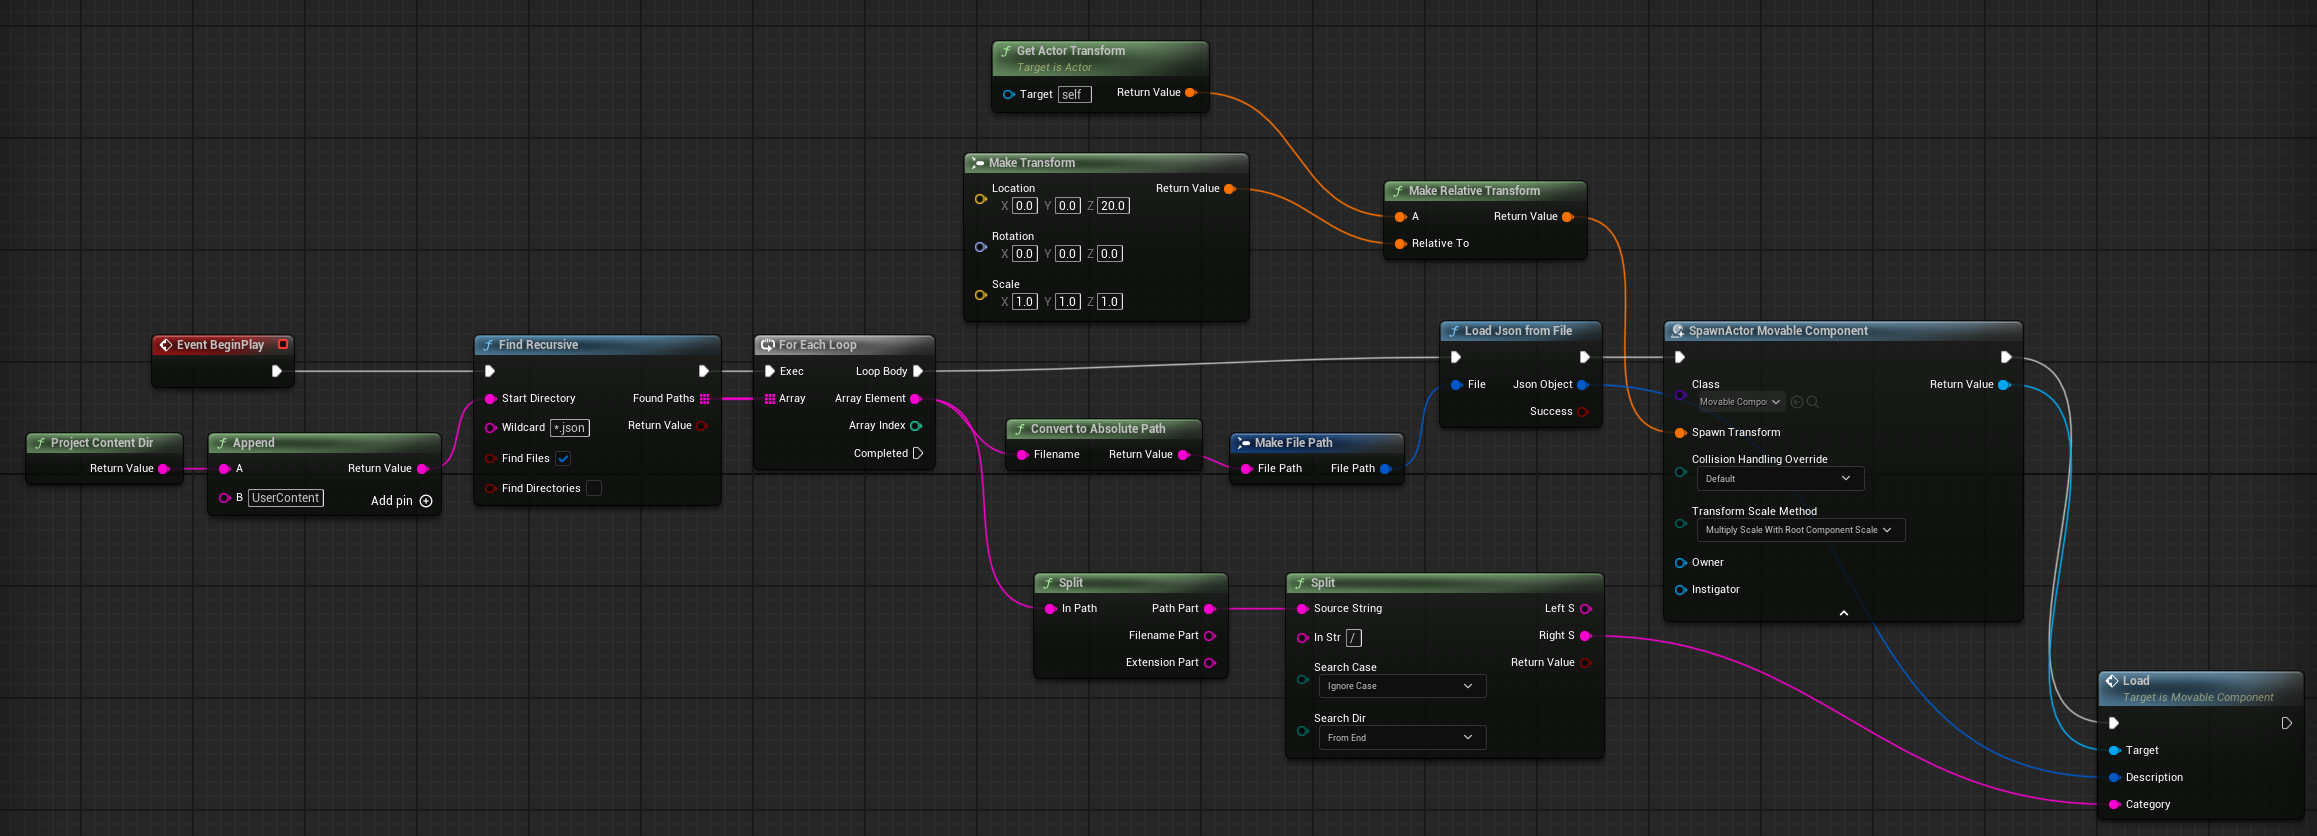
\includegraphics[width=1.0\textwidth]{Images/BasicLoadingBlueprint.png}
% 	\caption{Basic object loading blueprint}
% 	\label{fig:BasicLoadingBlueprint}
% \end{figure}

% The current loading scheme supports loading multiple meshes per object, which gives way to more complex models, such as GPUs with fans.
% Each mesh is expected to be a glTF 2.0 \cite{ISOIEC12113} model file, which is a modern format for 3D models, supporting PBR materials and animations.
% Each mesh can also be assigned a type, which is then used to assign specific functionality to it.
% For example, a mesh of type "Body" is treated as the main mesh of the object, while a mesh of type "Fan" could be rotated when the computer is turned on.

% \begin{figure}[H]
% 	\centering
% 		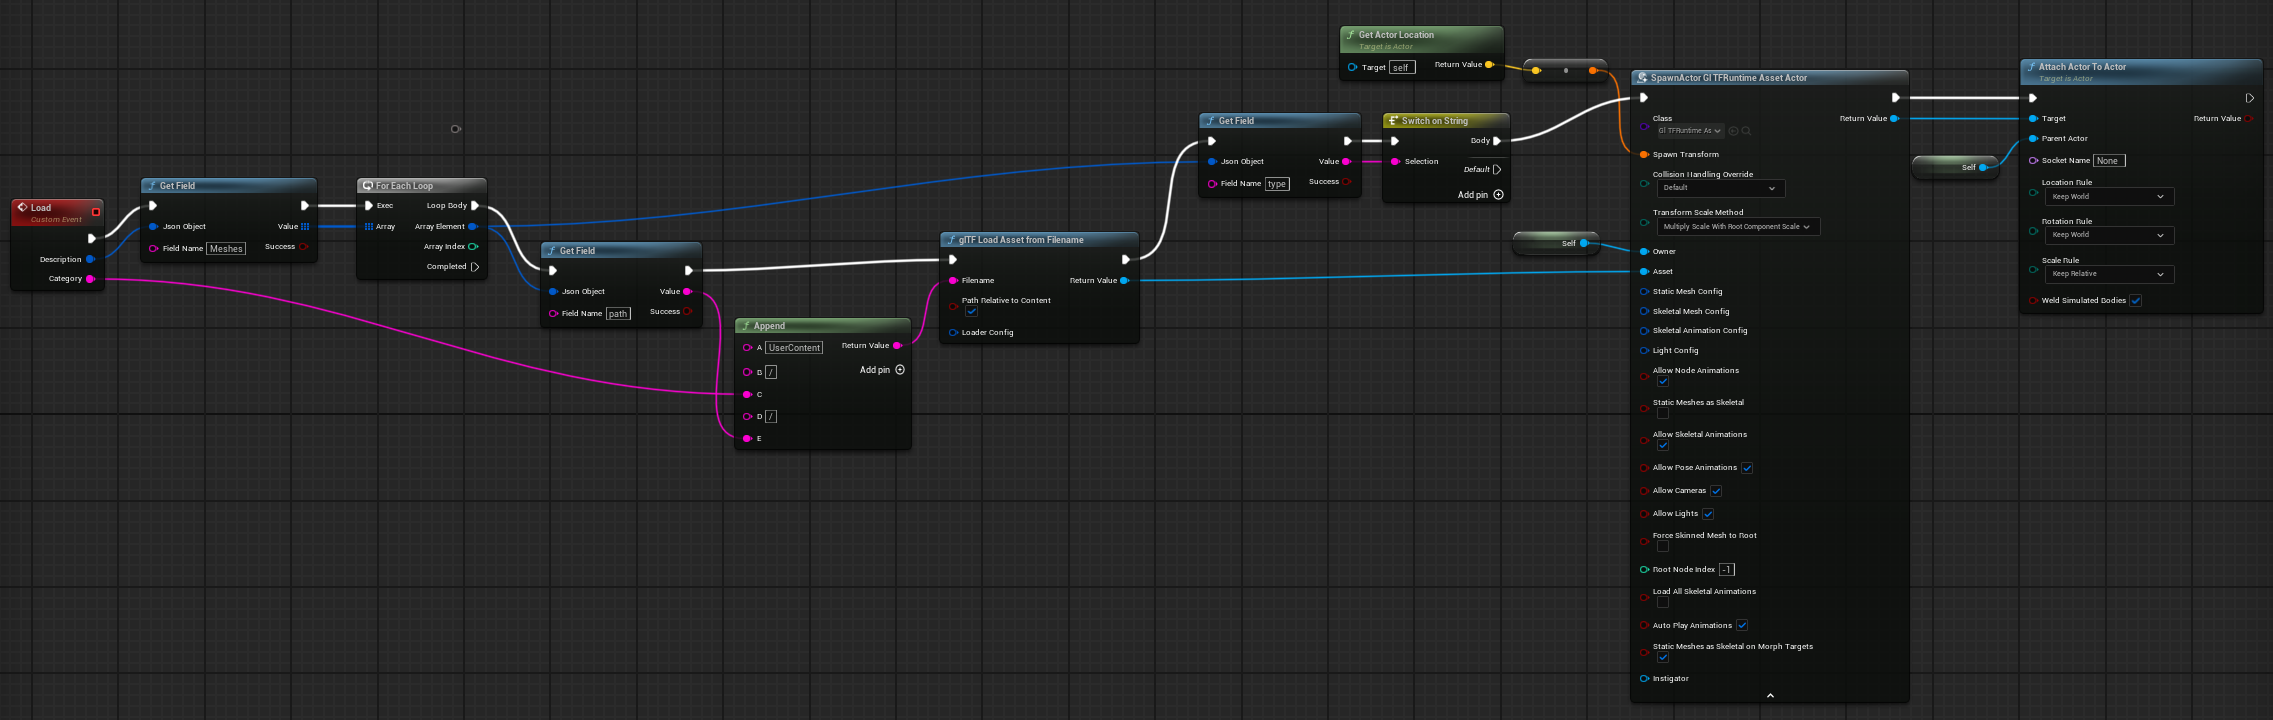
\includegraphics[width=1.0\textwidth]{Images/BasicObjectSelfPreparation.png}
% 	\caption{Basic object self-preparation blueprint}
% 	\label{fig:BasicObjectSelfPreparation}
% \end{figure}

% After placing this loading object in the scene and preparing appropriate description and model files, the object could be spawned in the scene at runtime.

% \begin{figure}[H]
% 	\centering
% 		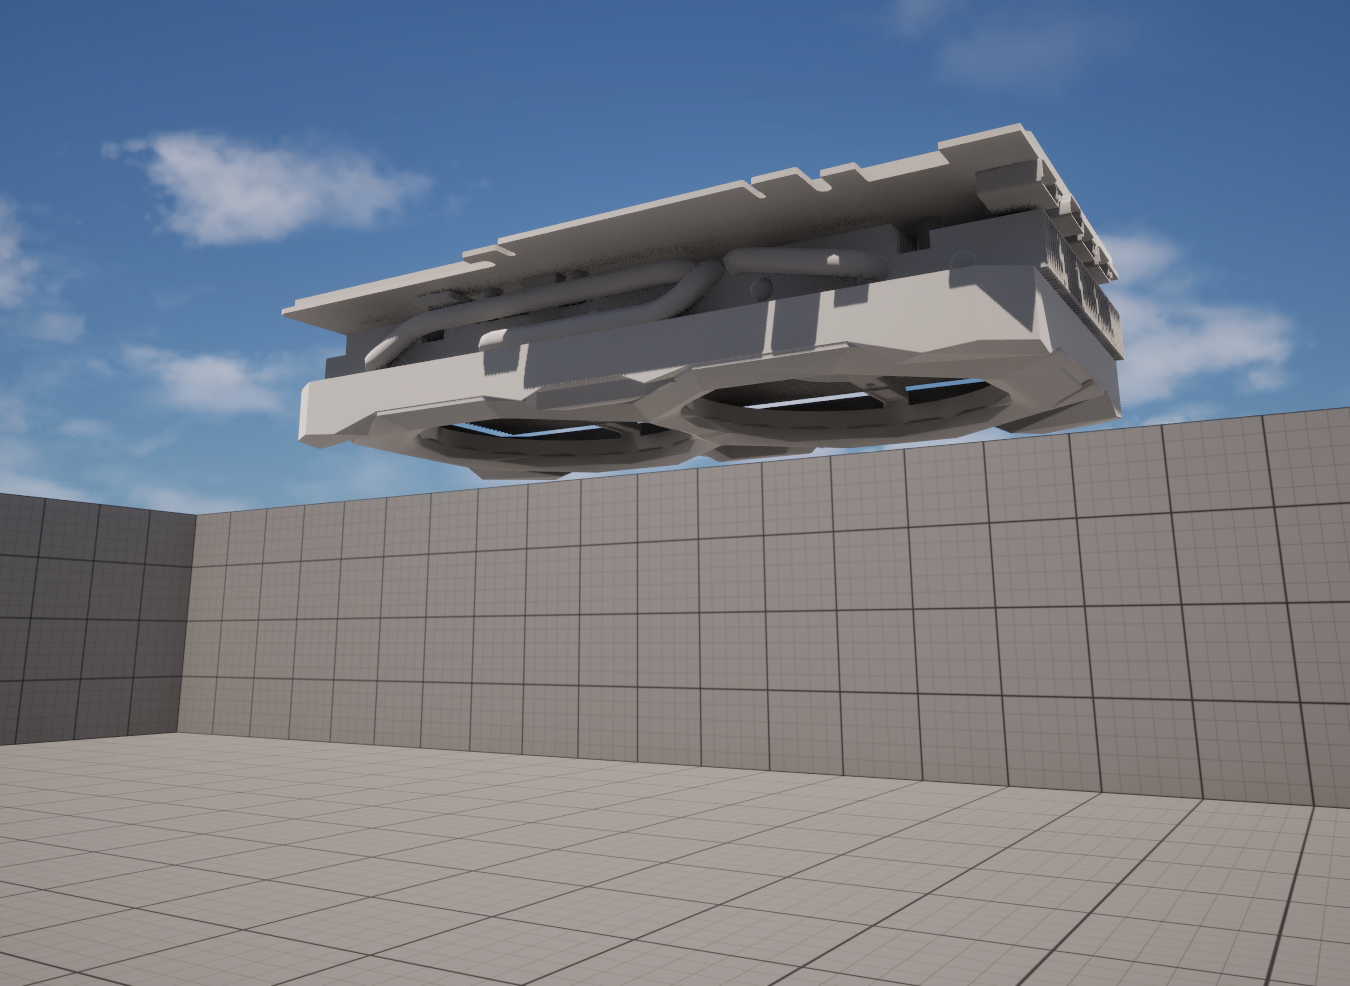
\includegraphics[width=0.7\textwidth]{Images/BasicGPULoaded.png}
% 	\caption{Basic GPU loaded blueprint}
% 	\label{fig:BasicGPULoaded}
% \end{figure}